\chapter{A practical demostration of a certificate lifecycle}

This chapter provides a simple guide for users on how to interact with the User Interface (UI) 
of the Identity Certificate Authority (IdenCA) system. The UI is designed to be intuitively 
allow users to perform essential operations. It's important to note that all cryptographic operations
requiring the use of the user's private key are handled in the browser, so it never leaves the 
user's device.

\section{Home page}
The Home Page serves as the starting point for interacting with the CA and is designed to show 
users the public key of the Certificate Authority (CA) and provide access to various functionalities.

On this page, users can:
\begin{itemize}
    \item View the Certificate Authority's public key.
    \item Download the public key for use in their applications.
    \item Copy the public key to their clipboard for easy access.
    \item Navigate to other important sections of the CA system.
\end{itemize}
\begin{figure}[h!]
    \centering
    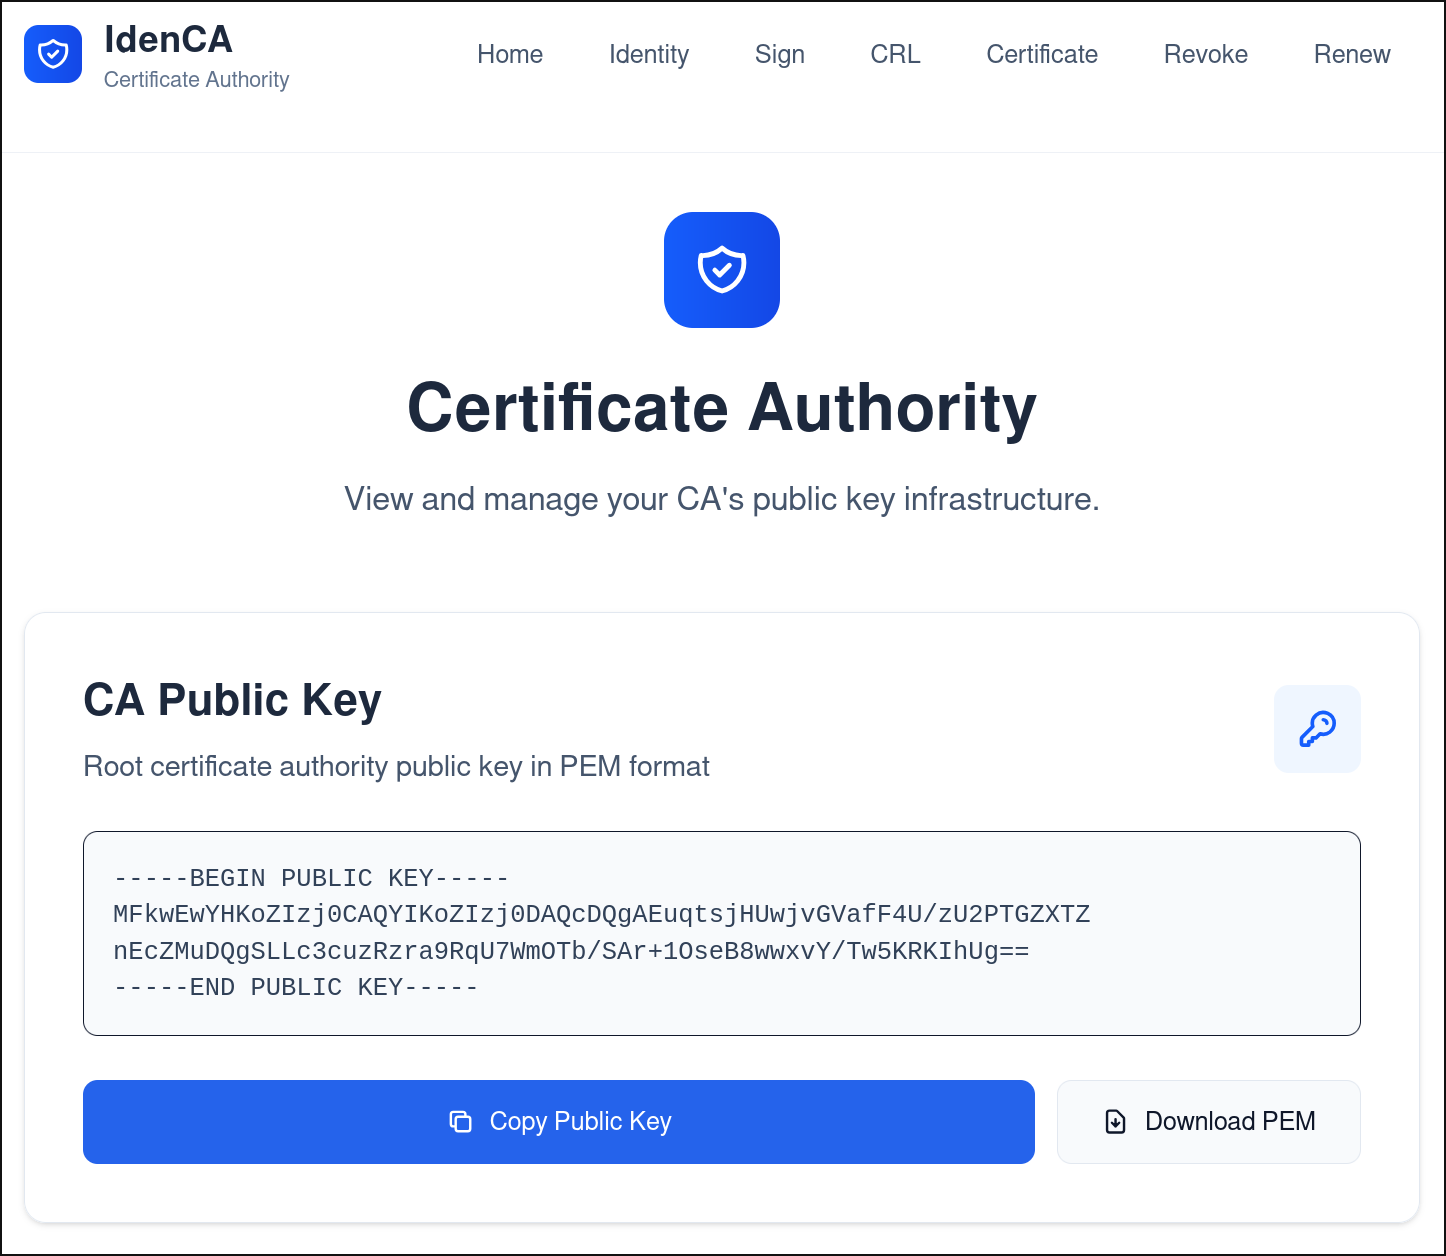
\includegraphics[keepaspectratio, width=0.6\textwidth]{Pic/1_ca_pub_key.png}
    \caption{Certificate Authority home page}
    \label{fig:homepage}
\end{figure}

\section{Creating a certificate}
To create a certificate, users must follow a series of steps that involve providing necessary 
information and completing a verification process. 
\subsection{Identity Commitment}
To begin the certificate request process users must first commit their identity:
\begin{itemize}
    \item Navigate to the "Identity" section.
    \item Enter email address in the designed field.
    \item Upload public key.
    \item Click the "Commit Identity" button to submit the request.
\end{itemize}
These steps register the user's identity with the CA and sends the verification challenge that must 
be signed in the next steps with the private key associated with the public key uploaded.
\begin{figure}[h!]
    \centering
    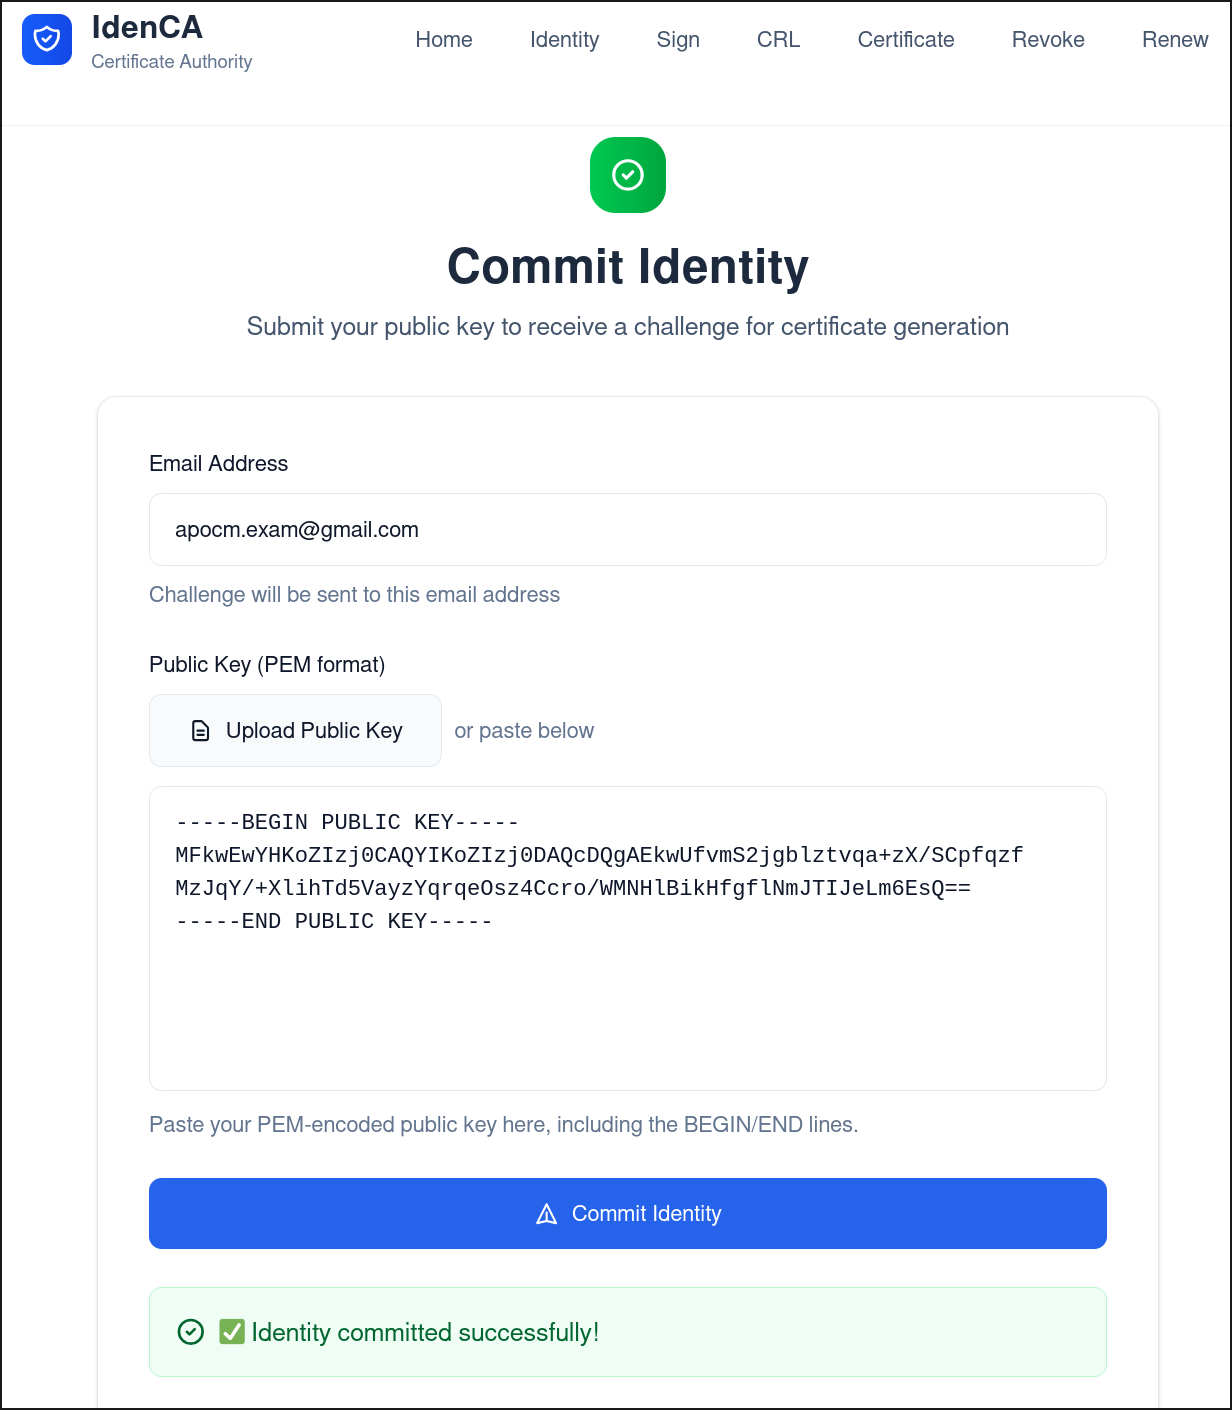
\includegraphics[keepaspectratio, width=0.6\textwidth]{Pic/2_identity_committed.png}
    \caption{Identity commitment page}
    \label{fig:identity-commitment}
\end{figure}

\subsection{Proving identity}
Once the identity commitment is created, users must copy the challenge sent by the CA to the provided
email address and sign it with their private key:
\begin{itemize}
    \item Navigate to the "Sign" section.
    \item Paste the challenge received from the CA into the designated field.
    \item Sign the challenge using the private key associated with the public key uploaded during 
            the identity commitment. This private key never leaves the browser.
    \item Click the "Sign \& Request Certificate" button to submit the signed challenge.
\end{itemize}
If the process is successful, the new certificate will be displayed on the screen and can be 
downloaded for use.
\begin{figure}[h!]
    \centering
    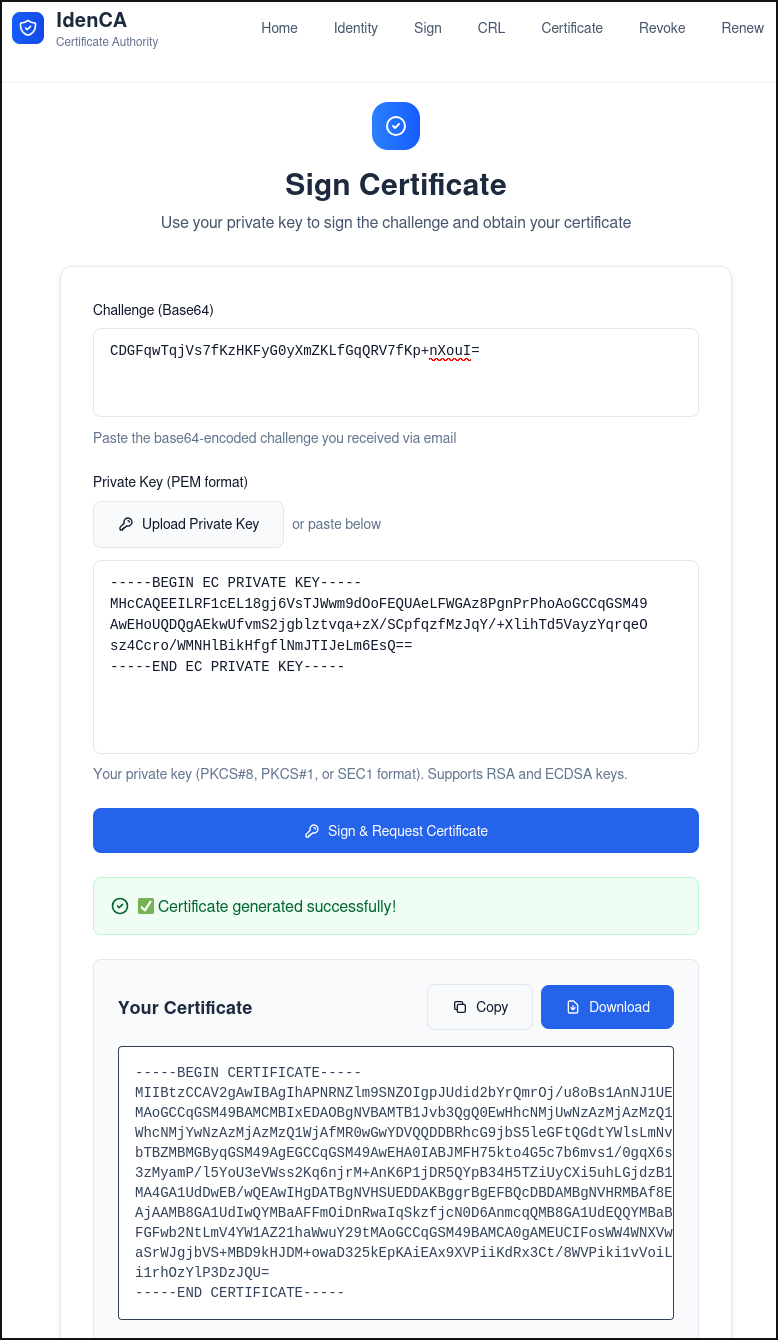
\includegraphics[keepaspectratio, width=0.6\textwidth]{Pic/4_certificate_generation.png}
    \caption{Identity proving and certificate generation flow}
    \label{fig:certificate-generation}
\end{figure}

\section{Certificate management}
\subsection{Viewing Certificates}
To view the details of a certificate, users can navigate to the "Certificate" section. Here, they can:
\begin{itemize}
    \item Upload a certificate.
    \item View the certificate's details, including its validity period, public key, and associated identity.
    \item If the certificate is valid and not expired, there will be two buttons:
        \begin{itemize}
            \item \textbf{Revoke Certificate}: To initiate the revocation process.
            \item \textbf{Renew Certificate}: To request a renewal of the certificate.
        \end{itemize}
\end{itemize}
\begin{figure}[h!]
    \centering
    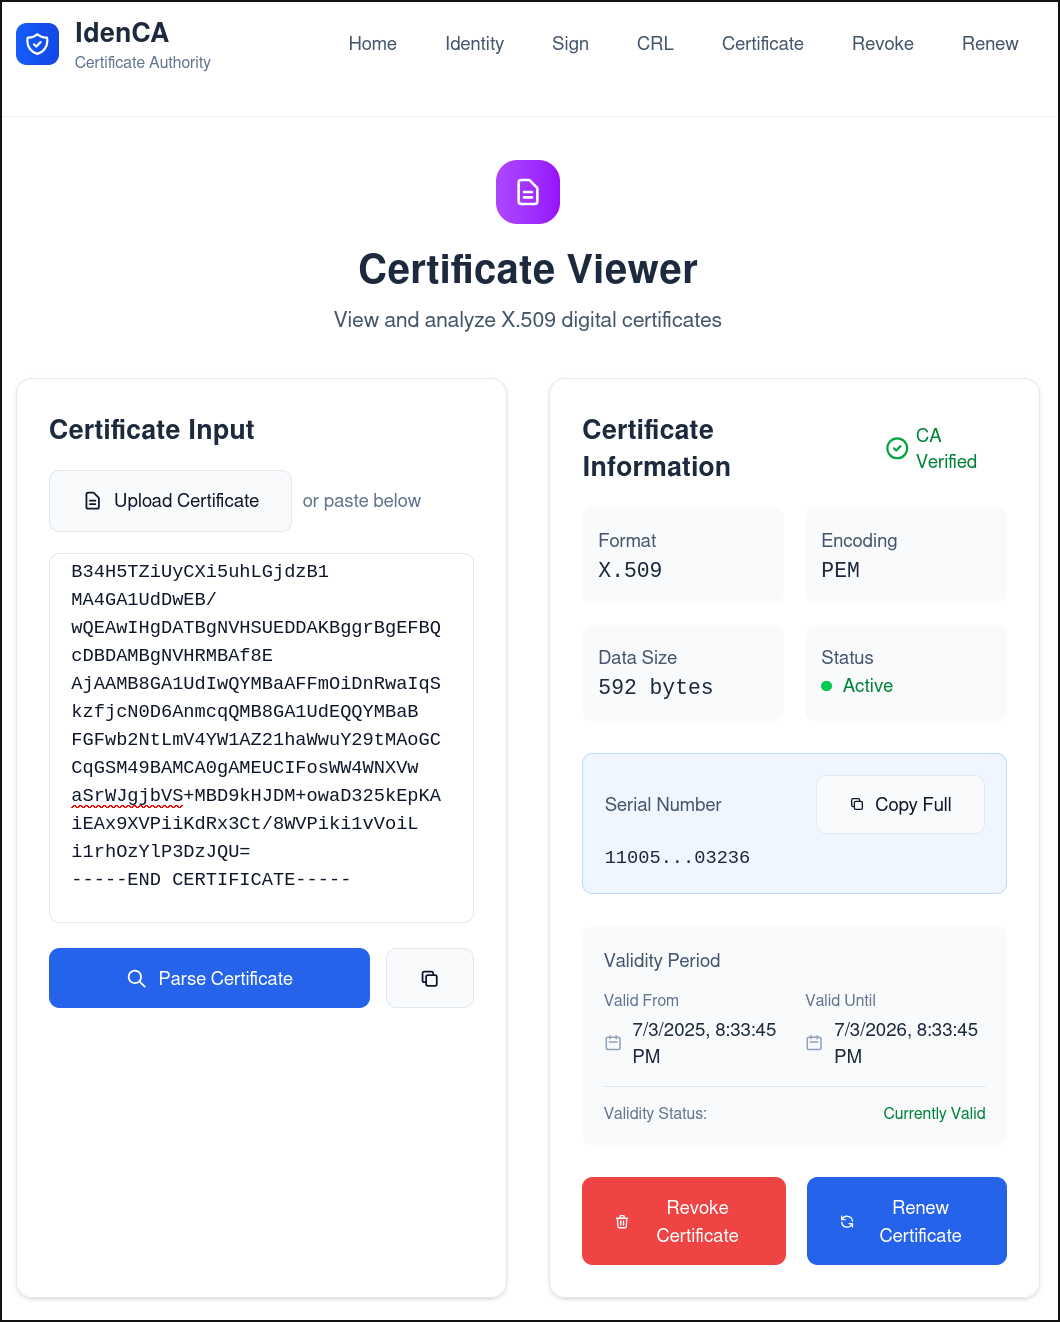
\includegraphics[keepaspectratio, width=0.6\textwidth]{Pic/5_certificate_view.png}
    \caption{Certificate view of a valid certificate}
    \label{fig:certificate-view-1}
\end{figure}

\subsection{Renewing a certificate}
Renewing a certificate requires the certificate's serial number and the 
private key associated with the certificate. Users can renew a certificate by:
\begin{itemize}
    \item Navigating to the "Renew" section.
    \item Entering the certificate's serial number and uploading the private key. A 
            nonce is automatically generated.
    \item Clicking the "Renew Certificate" button to submit the renewal request.
\end{itemize}
Alternatively, users can renew a certificate directly from the "Certificate" section by 
clicking the "Renew" button after viewing the certificate details.
In this case, the serial number will be automatically filled in.
\begin{figure}[h!]
    \centering
    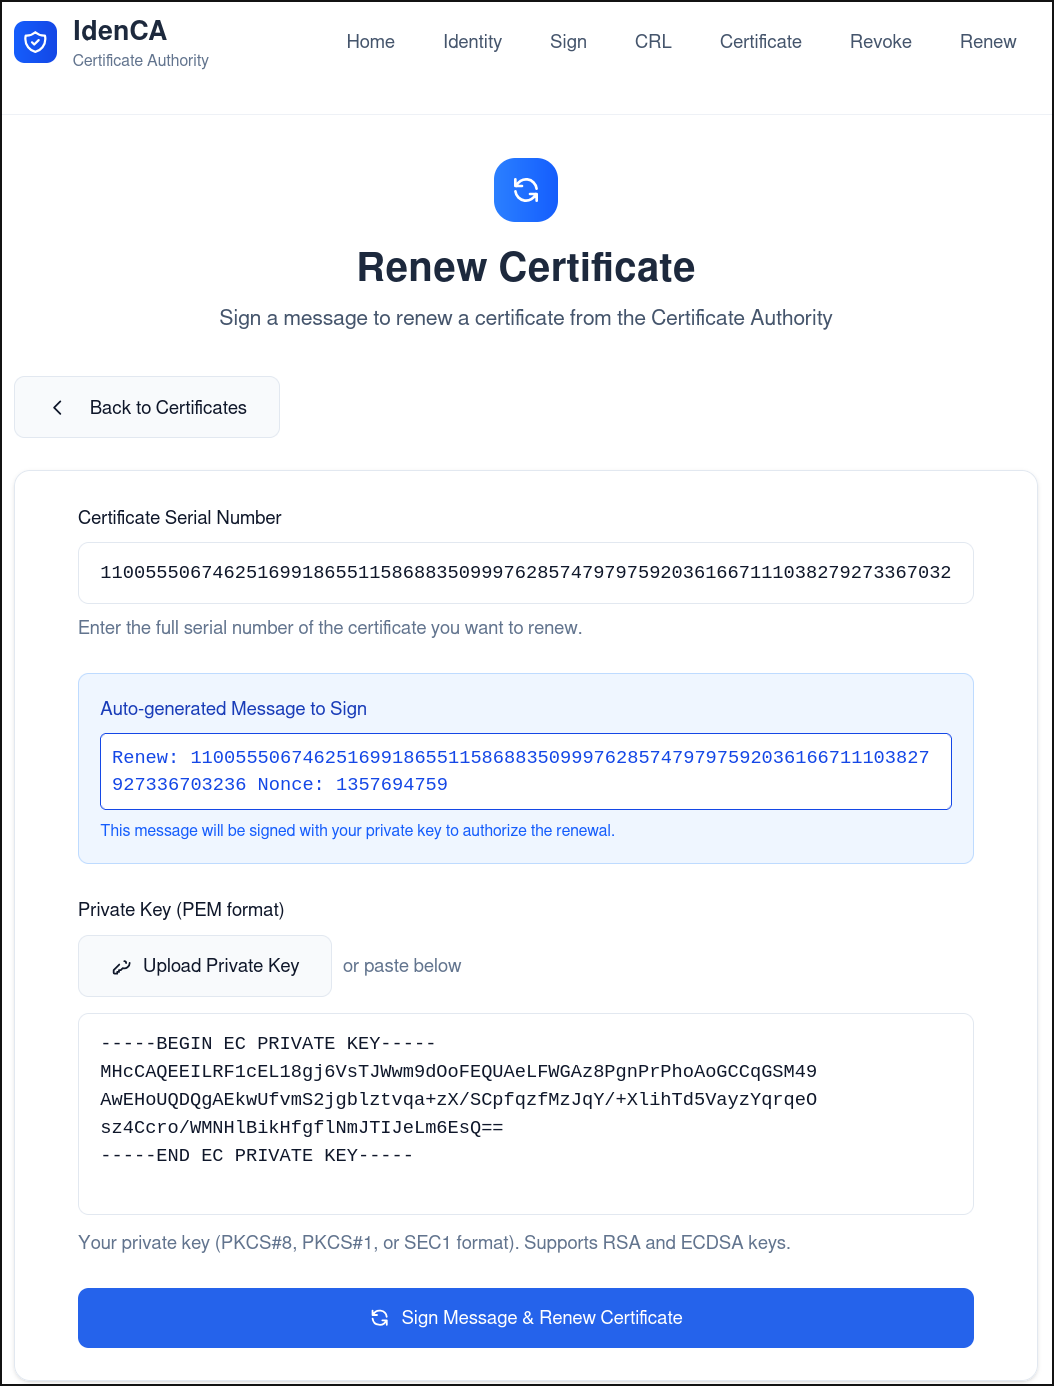
\includegraphics[keepaspectratio, width=0.5\textwidth]{Pic/6_renew_certificate.png}
    \caption{Certificate renewal page}
    \label{fig:certificate-renew}
\end{figure}
\begin{figure}[h!]
    \centering
    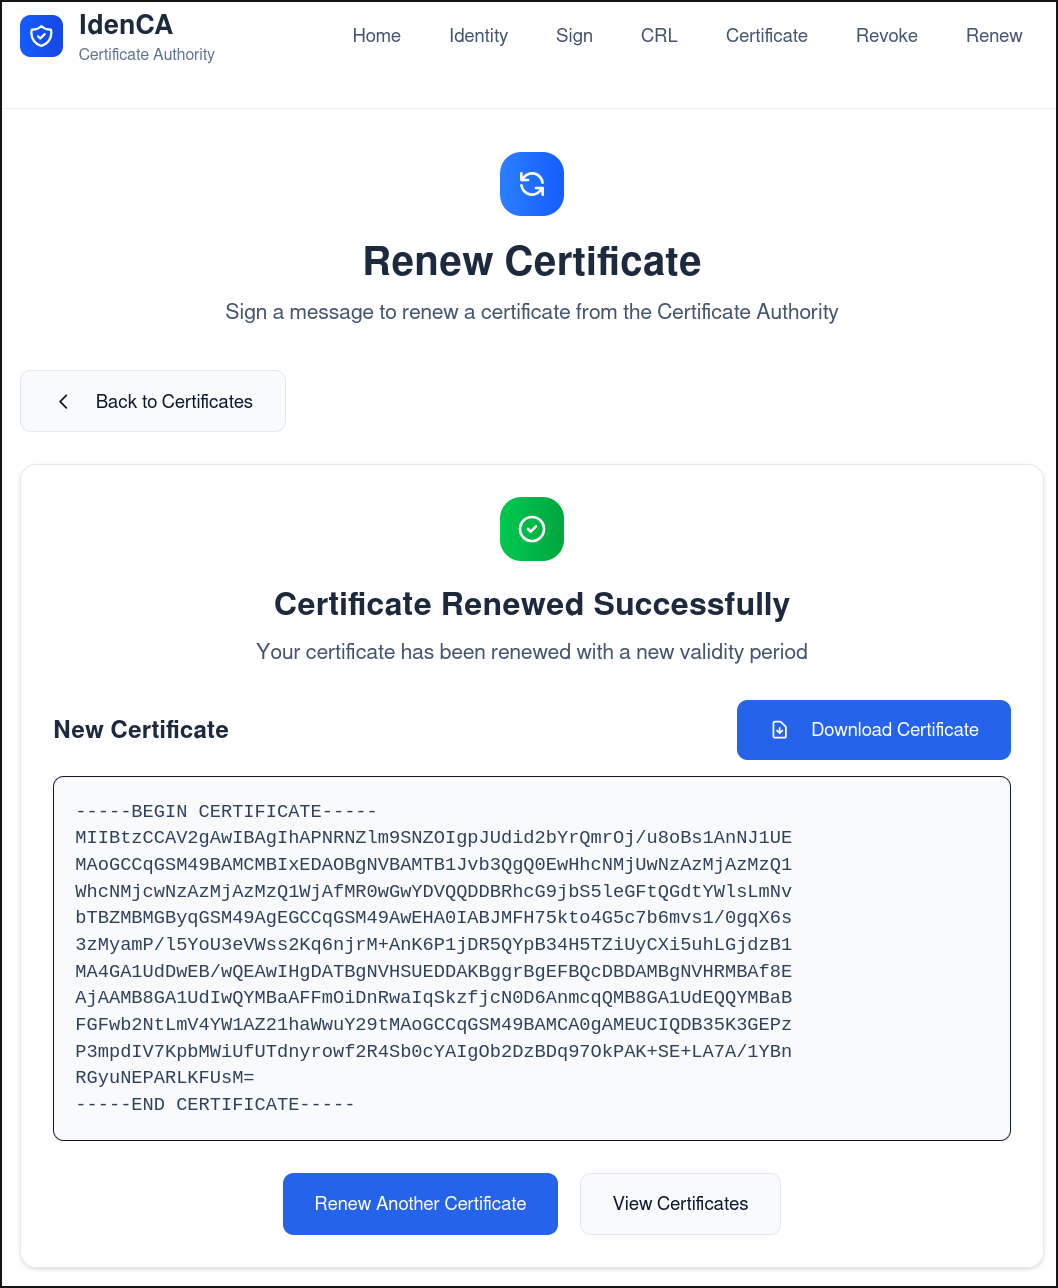
\includegraphics[keepaspectratio, width=0.6\textwidth]{Pic/7_renewed_certificate.png}
    \caption{Result of a successful certificate renewal}
    \label{fig:successful-renewal}
\end{figure}

\subsection{Revoking a Certificate}
For revoking a certificate, users need the certificate's serial number and the private key 
associated to the certificate. There are two ways to revoke a certificate:
\begin{itemize}
    \item Navigate to the "Revoke" section.
    \item Enter the certificate's serial number and upload the private key.
    \item Click the "Revoke Certificate" button to submit the revocation request.
\end{itemize}
Alternatively, users can revoke a certificate directly from the "Certificate" section by 
clicking the "Revoke" button after viewing the certificate details.
In this case, the serial number will be automatically filled in.
\begin{figure}[h!]
    \centering
    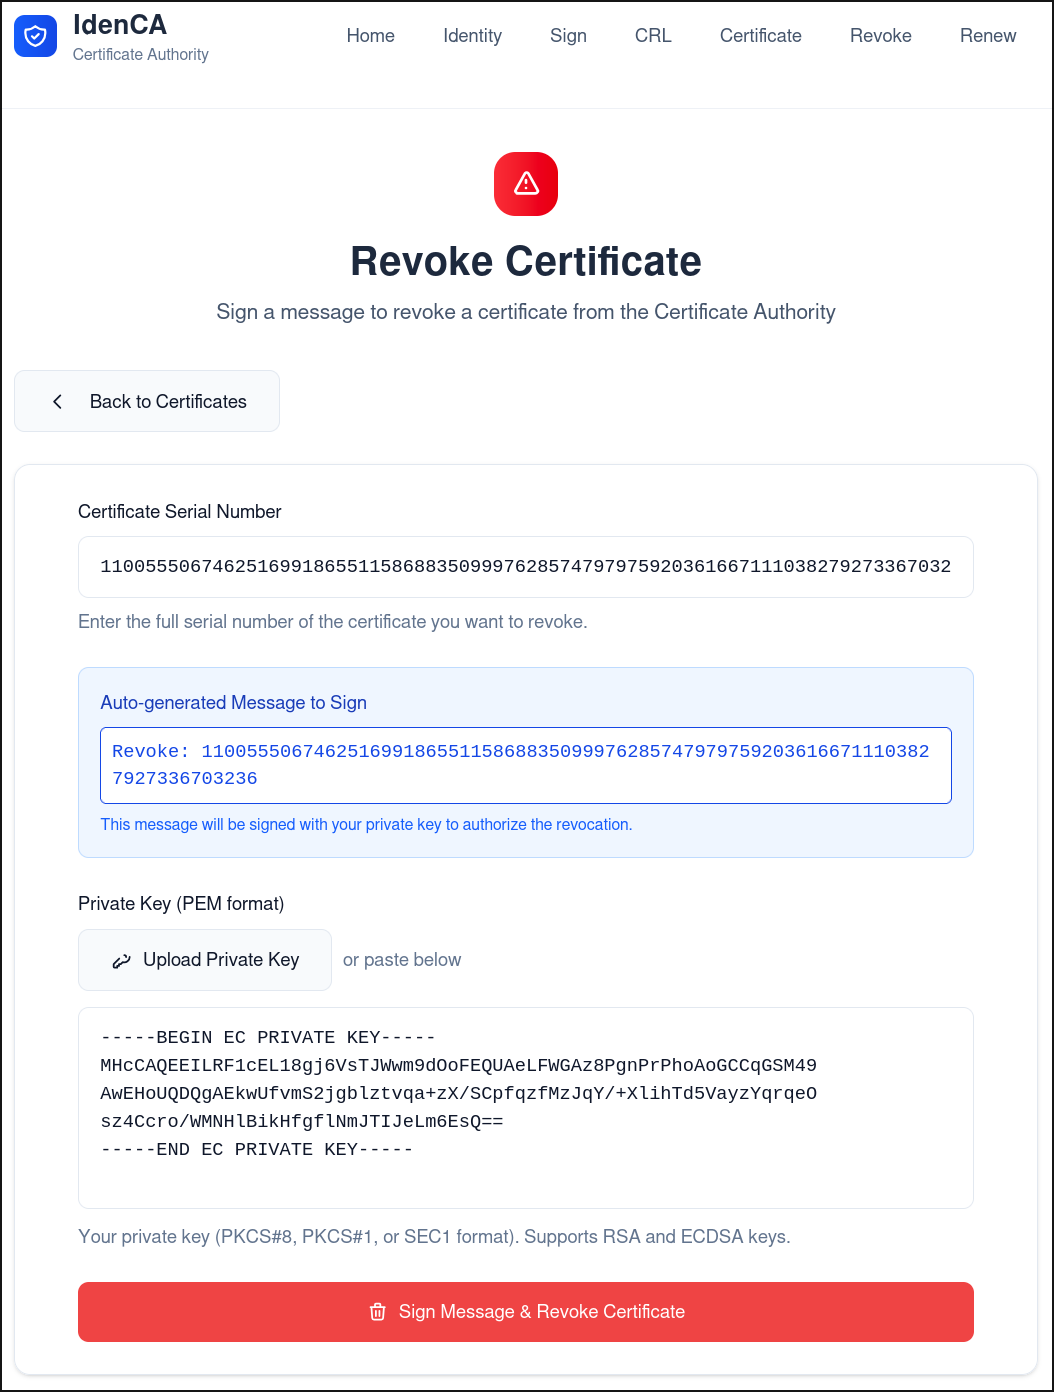
\includegraphics[keepaspectratio, width=0.6\textwidth]{Pic/9_revoke_certificate.png}
    \caption{Certificate revocation page}
    \label{fig:revocation-flow}
\end{figure}

\section{Certificate Revocation List (CRL)}
Visit the "CRL" section to view the Certificate Revocation List. 
This list contains all certificates that have been revoked by the CA. 
\begin{figure}[h!]
    \centering
    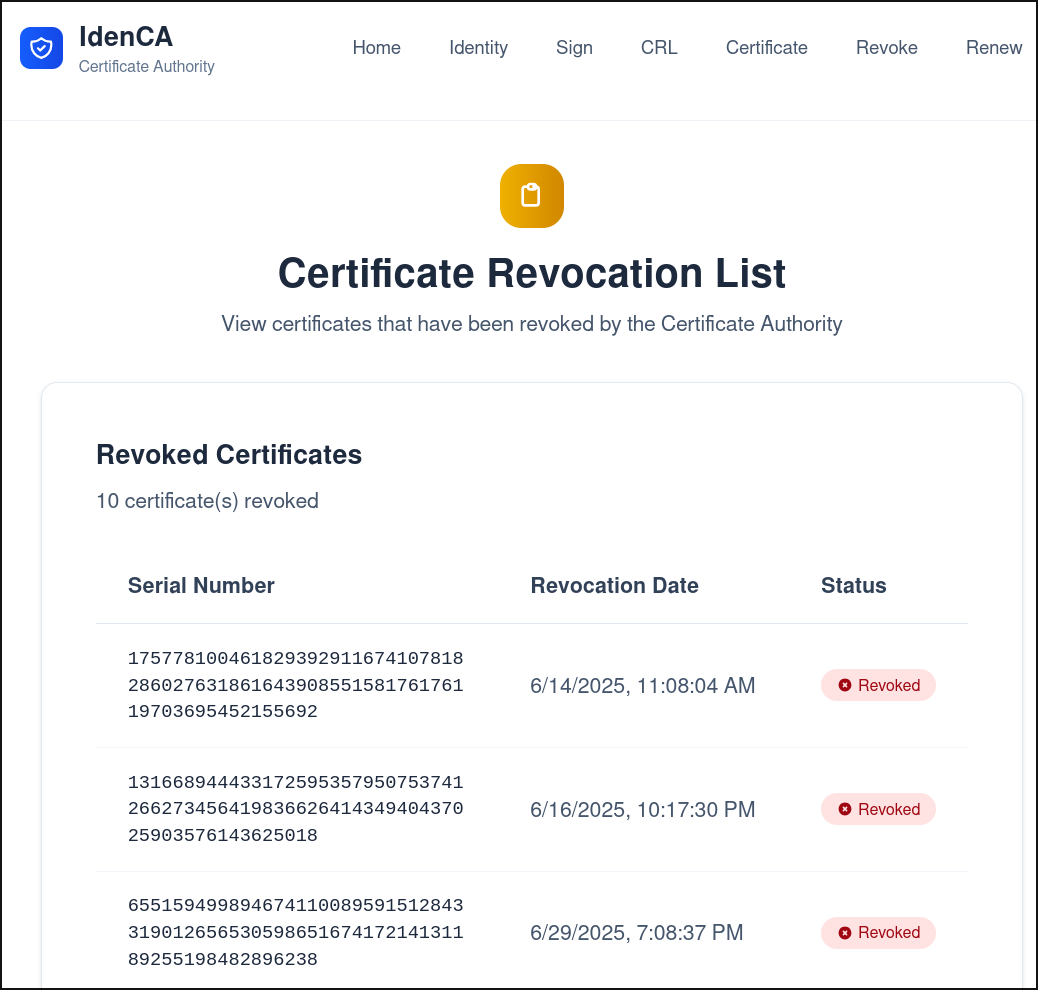
\includegraphics[keepaspectratio, width=0.6\textwidth]{Pic/11_crl.png}
    \caption{Revoked certificates page}
    \label{fig:crl-page}
\end{figure}


This guide covers the basic functionalities of the UI. For advanced features or troubleshooting, refer to the system documentation or contact the administrator.